\documentclass[10pt,a4paper,openany,notitlepage]{article}
\usepackage[latin1]{inputenc}
%\usepackage[italian]{babel}
\usepackage{hyperref}
\hypersetup{
    colorlinks,
    citecolor=gray,
    filecolor=red,
    linkcolor=blue,
    urlcolor=blue
}
\usepackage{amsmath}
\usepackage{geometry}
%\usepackage{xcolors}
\usepackage{graphicx}
\usepackage{pdflscape}
%\usepackage{lscape}
\usepackage{amsfonts}
\usepackage{amssymb}
\usepackage{listings}
\lstset{%
	commentstyle=\color{green},
	frame=single,
	keepspaces=true,
	keywordstyle=\color{blue},
	numbers=left,
	numberstyle=\tiny\color{gray},
	rulecolor=\color{black},
	columns=flexibile
}
\author{Davide Polonio, Alessandro Bari}
\title{Progetto di Basi di Dati 2015}
\begin{document}
\maketitle
\newpage
\tableofcontents
\newpage

\section{Progettazione Concettuale}

\subsection{Studio di fattibilit\`a} 

\paragraph*{Priorit\`a di realizzazione}
Come priorit\`a di realizzazione abbiamo deciso di implementare le seguenti feature:
\begin{itemize}
\item Percentuale di sconto basata sul numero di acquisti effettuato da un acquirente iscritto al servizio.
\item Gestione degli ordini e delle fatture del negozio, oltre che degli scontrini e delle vendite effettuate riferite agli iscritti.
\item Gestione e organizzazione dei turni per i dipendenti.
  \item Catalogazione prodotti in diverse categorie (a cui appartengono diverse percentuali di sconto).
\end{itemize}

\subsection{Raccolta e analisi dei requisiti}

\subsubsection{Analisi dei requisiti}
Per i clienti \textbf{iscritti} identificati da un codice, vogliamo tenere conto dell'identit\`a e dei suoi acquisti effettuati.



Ogni \textbf{prodotto} \`e identificato da un codice, vogliamo tenere conto delle informazioni base e della quantit\`a disponibile e catalogarlo in una delle cinque \textbf{categorie}, identificate come: porcellane, pentolame, liste nozze, stoffe, stoviglie.


Ad ogni categoria sono associati possibili \textbf{sconti} in base ad una distribuzione per livelli e con una relativa percentuale.


I \textbf{dipendenti}, responsabili ognuno di una singola categoria, sono identificati da un codice e sono organizzati per turni.


Vogliamo tener conto degli ordini di merce ai \textbf{fornitori} con rispettive \textbf{fatture}. \\


\subsubsection{Glossario dei termini}
\begin{center}
\begin{tabular}{ l | p{5cm} | p{3cm} | p{3cm} }
%\hline

\textbf{Termine} & \textbf{Descrizione} & \textbf{Sinonimi} & \textbf{Collegamenti} \\ \hline

Iscritto & Compratore abituale iscritto a questa lista per avere diritto a sconti speciali. Pu\`o essere un dipendente. & Cliente abituale & Acquisto, Scontrino \\ \hline

Scontrino & Scontrino attestante lo storico degli acquisti. & Storico, acquisto & Iscritto, Prodotto \\ \hline

Categoria & Cinque insiemi di prodotti. Un prodotto pu\`o appartenere ad un'unica categoria. Ogni categoria ha il suo univoco responsabile. & & Sconto, Dipende, Prodotto. \\ \hline

Sconto & Spetta solamente al cliente iscritto. Per ogni categoria esistono diversi livelli in base agli acquisti, a cui corrisponde una percentuale di sconto. & & Categoria. \\ \hline

Dipendente & Responsabile di una singola categoria. Pu\`o essere un cliente ma non un fornitore. & Responsabile & Categoria \\ \hline

Prodotto & Ogni prodotto pu\`o appartenere ad una sola categoria. & Oggetti, Prodotto ordinati o acquistati & Categoria, Fattura, Scontrino \\ \hline

Fattura & Pi\`u unit\`a di prodotto possono essere ordinate a fornitori diversi. Modifica il campo quantit\`a disponibile di prodotto. & Ordine & Fornitore, Prodotto \\ \hline

Fornitore & Forniscono i prodotti attraverso gli ordini. Un fornitore non pu\`o essere un cliente e pu\`o fornire prodotti di diverse categorie & & Ordine \\


%\hline
\end{tabular}
\end{center}


\subsubsection{Schema Concettuale}

\paragraph*{Lista delle Entit\`a}

\begin{itemize}

\item \underline{Dipendente}: lista dei dipendenti del negozio.
  
  \begin{itemize}

  \item Codice dipendente (PK)
    
  \item Informazioni: dati anagrafici e di recapito del dipendente
    \begin{itemize}
    \item Nome
    \item Cognome
    \item Data di nascita
    \item Codice Fiscale
    \item Telefono
    \item E-mail
    \end{itemize}
    
  \item Indirizzo:
    \begin{itemize}
    \item Via
    \item Numero
    \item Citt\`a
    \end{itemize}

  \end{itemize}

\item \underline{Categoria}: insieme di prodotti
  \begin{itemize}
  \item Nome Categoria (PK)
  \item Responsabile (FK)
  \end{itemize}

\item \underline{Sconto}: entit\`a destinata a contenere tutti i gradi di sconto di tutte le categorie
  \begin{itemize}
  \item Livelli (PK)
  \item Categorie (FK)
  \item Tetto Max
  \end{itemize}

\item \underline{Prodotto}: lista di tutti i prodotti in vendita
  \begin{itemize}
  \item Codice Prodotto (PK)
  \item Quantit\`a
  \item Percentruale iva
  \item Categoria (FK)
  \end{itemize}

\item \underline{Specifica}: descrizione base sul prodotto
  \begin{itemize}
  \item Codice Prodotto (FK)
  \item Descrizione
  \item Nome
  \item Foto
  \end{itemize}

\item \underline{Fattura}: contenente tutti gli attestati di avvenuto ordine per un certo numero di prodotti
  \begin{itemize}
  \item Codice Fattura (PK)
  \item Codice Prodotto (FK)
  \item Quantit\`a
  \item Data
  \item Fornitore (FK)
  \end{itemize}

\item \underline{Fornitore}: lista di tutti i venditori da cui il negozio acquista i prodotti
  \begin{itemize}
  \item Nome (PK)
  \item Contatto
    \begin{itemize}
    \item Fax
    \item Telefono
    \item E-mail
    \end{itemize}

  \item Indirizzo:
    \begin{itemize}
    \item Via
    \item Provincia
    \item Citt\`a
    \end{itemize}
  \end{itemize}
  Di cui sono presenti le seguienti generalizzazioni:
  \begin{itemize}
  \item \underline{Artigiano}: Fornisce prodotti fatti a mano
  \item \underline{Grossista}: Fornisce prodotti all'ingrosso
  \end{itemize}

\item \underline{Scontrino}: registro di tutti le vendite effettuate ai clienti iscritti
  \begin{itemize}
  \item Codice Scontrino (PK)
  \item Data (PK)
  \item Quantit\`a
  \item Codice Prodotto (FK)
  \end{itemize}

\item \underline{Cliente}: lista dei clienti, di cui abbiamo creato la seguente generalizzazione parziale:
  \begin{itemize}
  \item \underline{Iscritto}: clienti iscritti
    \begin{itemize}
    \item Codice Iscritto (PK)
    \item Indirizzo:
      \begin{itemize}
      \item Via
      \item Provincia
      \item Citt\`a
      \end{itemize}

    \item Contatto
      \begin{itemize}
      \item Fax
      \item Telefono
      \item E-mail
      \end{itemize}

    \item Identit\`a
      \begin{itemize}
      \item Nome
      \item Cognome
      \end{itemize}

    \end{itemize}
  \end{itemize}
  
\end{itemize}


\subsubsection{Lista delle Relazioni}

\begin{itemize}

\item \underline{Responsabile}: relazione tra Dipendente-Categoria.
  \begin{itemize}
  \item Presenza di due attributi:
  \begin{itemize}
  \item Turno
  \item Data di inizio
  \end{itemize}
  La cardinalit\`a \`e (1,1) in quanto ogni dipendente \`e responsabile solamente di una categoria e vi lavora in una determinata data e in un rispettivo turno.

  \end{itemize}

\item \underline{Scaglioni}: relazione tra Categoria-Sconto. \`E una cardinalit\`a (0,N) da Categoria $\to$ Sconto, mentre la cardinalit\`a risulta essere (1,N) da Sconto $\to$ Categoria. \newline
Ogni Categoria presenta dei diversi scaglioni di sconti in base al livello di acquisto.

\item \underline{Appartenenza}: relazione tra Categoria-Prodotto. Da Prodotto $\to$ Categoria abbiamo imposto una cardinalit\`a di tipo (1,1) in quanto un Prodotto deve appartenere a una ed una sola Categoria. \newline
  La cardinalit\`a \`e (0,N) da Categoria $\to$ Prodotto in quanto una nuova categoria pu\`o non contenere prodotti.\newline
  Si prenda l'esempio della Categoria \textit{Liste Nozze}: quando il negozio non sta svolgendo nessuna attivit\`a per matrimoni la categoria \textit{Lista Nozze} risulter\`a essere vuota. %DA FARE FRAMEBOX PERCHÈ ESEMPIO

\item \underline{Definito}: relazione tra Prodotto-Specifica. La cardinalit\`a tra Prodotto e Specifica \`e (1,1) in quanto ogni prodotto ha una singola specifica.

\item \underline{Registrato}: relazione tra Fattura-Prodotto. Da Prodotto $\to$ Fattura abbiamo una relazione di tipo (1,N) in quanto un prodotto deve risultare registrato in una fattura. \newline
  Da Fattura $\to$ Prodotto la cardinalit\`a \`e (1,N) perch\`e una fattura per essere emessa deve contenere uno o pi\`u prodotti

\item \underline{Emesso}: relazione tra Fattura-Fornitore. Da fattura a fornitore la cardinalit\`a \`e (1,1): una fattura pu\`o essere solamente emessa da un singolo fornitore. \newline
  Da Fornitore $\to$ a Fattura \`e (1,N) in quanto viene memorizzato solamente un fornitore che abbia almeno emesso una o pi\`u fatture al negozio.

\item \underline{Certifica}: relazione tra Prodotto-Scontrino. Ha cardinalit\`a (0,N) in Prodotto $\to$ Scontrino siccome un prodotto pu\`o esser stato acquistato da zero a pi\`u volte, invece da Scontrino $\to$ Prodotto vi \`e una cardinalit\`a (1,N), uno scontrino infatti certifica almeno un prodotto.

\item \underline{Ottiene}: relazione tra Scontrino-Cliente. In Scontrino $\to$ Cliente vi \`e una relazione (1,1) in quanto uno scontrino si riferisce ad un singolo acquirente, mentre tra Cliente $\to$ Scontrino vi \`e una relazione (1,N) ne consegue che un cliente pu\`o fare molti acquisti. Un cliente per essere definito tale deve almeno aver compiuto un acquisto.
  
\end{itemize}

%Passi successivi: Schema, Progettazione logica, Schema Normalizzato.

\newpage
\subsection{Schema E-R}

\begin{figure}[h!]
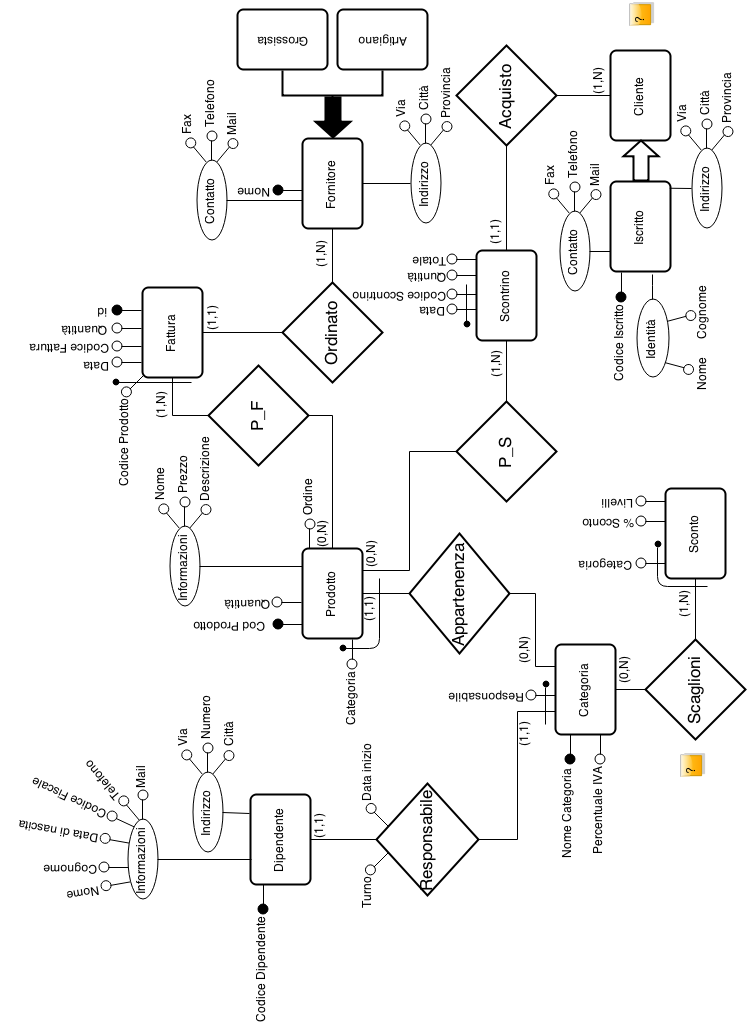
\includegraphics[scale=0.52]{include/progettazioneConcettuale/schemaER/output}
\end{figure}



\end{document}
